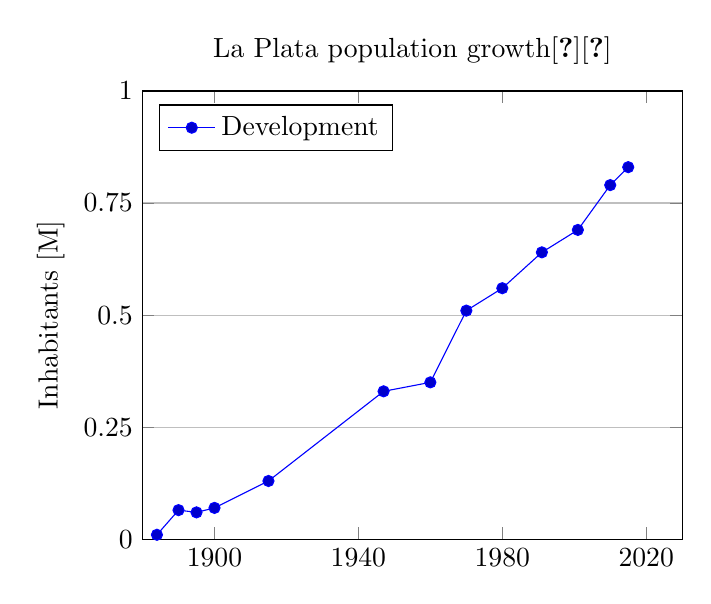
\begin{tikzpicture}[>=latex]
	\begin{axis}[
			title={La Plata population growth\cite{Population.City:LaPlata}\cite{Wikipeda:LaPlataHistory}},
			style={/pgf/number format/1000 sep=},
			ylabel={Inhabitants [M]},
			xmin=1880, xmax=2030,
			ymin=0, ymax=1,
			xtick={1900,1940,1980,2020},
			ytick={0,0.25,0.5,0.75,1},
			legend pos=north west,
			ymajorgrids=true
		]				
		\addplot coordinates {
				(1884,0.01)(1890,0.065)(1895,0.06)(1900,0.07)(1915,0.13)(1947,0.33)(1960,0.35)(1970,0.51)(1980,0.56)(1991,0.64)(2001,0.69)(2010,0.79)(2015,0.83)
			};
		
		\legend{Development}				
	\end{axis}
\end{tikzpicture}	
